\vspace{-3cm}\chapter{实验3. 长度n的子序列最大乘积}

\section{3.1 实验题目}
从文件中输入一个数字序列字符串,计算给定的长度n的子序列中的最大乘积值。

例如:如果输入“1027839564”,指定长度为3的最大子序列乘积值为 270(9*5*6);指定长度为5的最大子序列乘积值为7560(7*8*3*9*5)。

备注:
\begin{enumerate}
    \item 数字序列字符串的最大长度maxLength 的范围为:[1..1000];
    \item n 的取值范围为[1..maxLength-1];
    \item 程序要注意处理边界情况;
    \item 程序的输入数据必须从文件中读取。
\end{enumerate}

下图为一个长度为 1000 的字符串数字序列,在这个序列中,长度为 4 的最大子序列乘积为 5832(9*9*8*9). 
\begin{figure}[H]
    \centering
    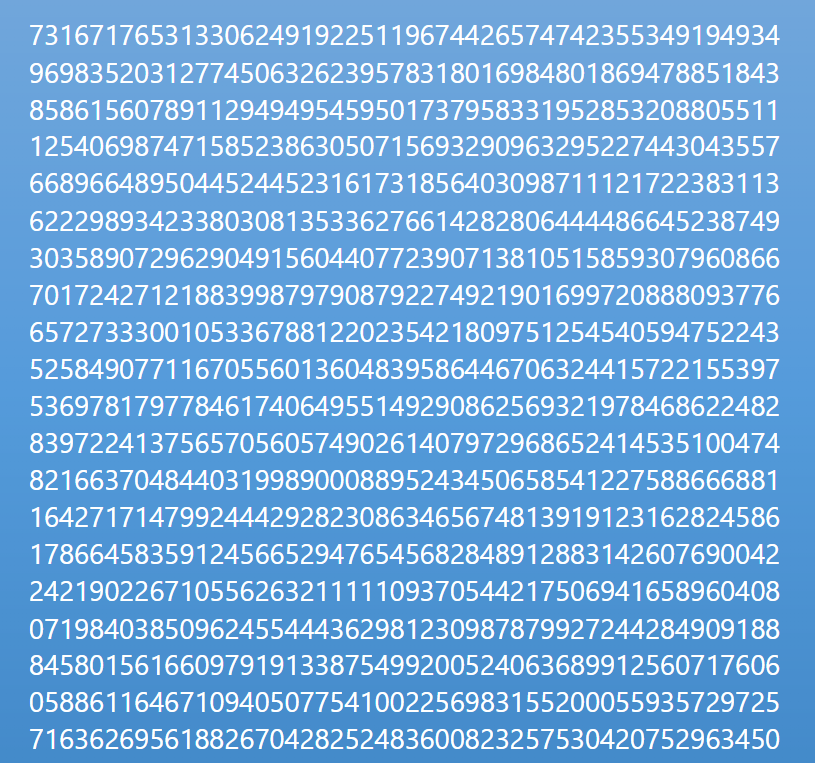
\includegraphics[width = 0.8\textwidth]{../pic/3/3.0.png}
\end{figure}